\section{DeploymentUnit(UAV)}\label{sec:DeploymentUnit(UAV)}

\subsection{Design}

\todobox{Victor: image of the deployment system.  }
\textbf{\begin{figure} \centering
  {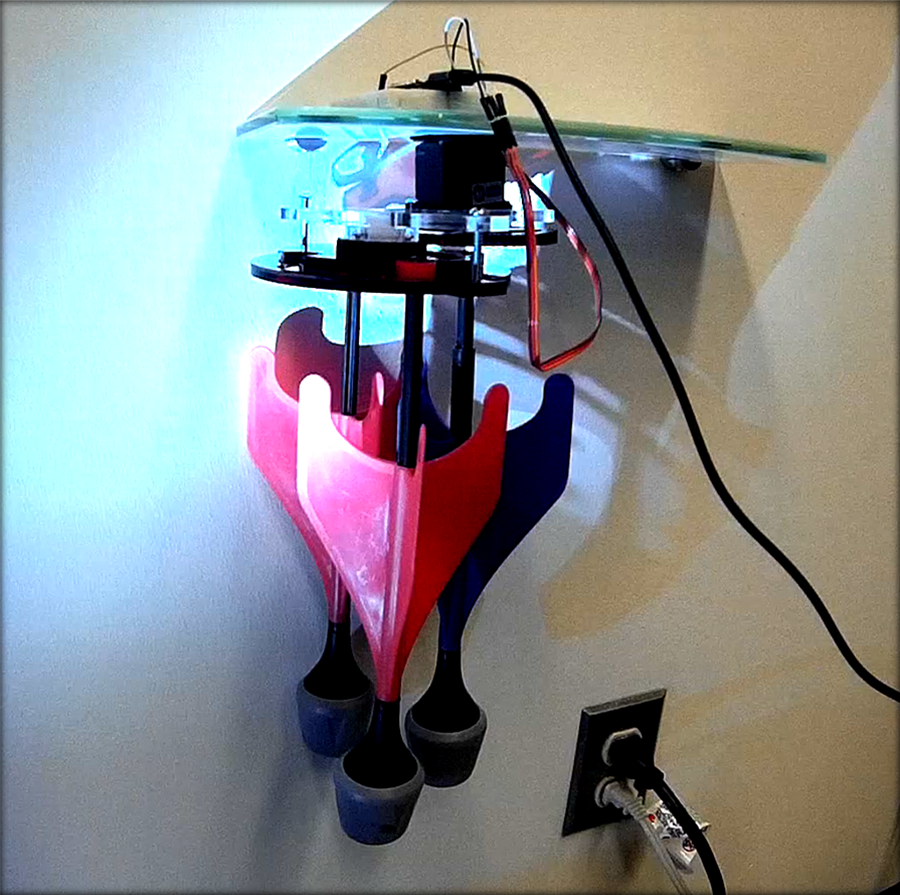
\includegraphics[width=\columnwidth]{deploment_mech.png}}
 \caption{Deployment mechanism for smart darts} 
 \label{fig:TradvsAutoDrop}
\end{figure}}
\todobox{An: I want to know about the deployment unit.  }

\subsection{Experiment}


\subsubsection{Autonomous drop demonstration and accuracy}

The current drone can place the SmartDart within $\pm1$ m of the desired location.  This inaccuracy is 
1)     There are often features (rocks, water, etc.) that require this amount of error from theoretically assigned locations,
2)     some survey designs include a random placement component to improve noise cancellation,
3)     this error minimally perturbs  the data since seismic waves travel at 600 m/s in near surface, so a one-meter inaccuracy equates to $\approx$1.6 ms delay,
4)     the response of a receiver to seismic vibrations is an average over a number of meters.

The critical factor is to know exactly (within 10 cm accuracy)  the geophone location. Knowledge of this exact location allows corrections for the possible jitter in arrival times of the signal due to inaccuracy of placement.


Exp 4: Automatic drop from drone, accuracy in placement

\todobox{AN:  Need figure for accuracy of placement for drone drop}



\subsubsection{Height vs. penetration depth}
Exp 5: Height vs. penetration depth

\todobox{AN:  Need figure for accuracy of placement for drone drop}

\textbf{\begin{figure} \centering
  {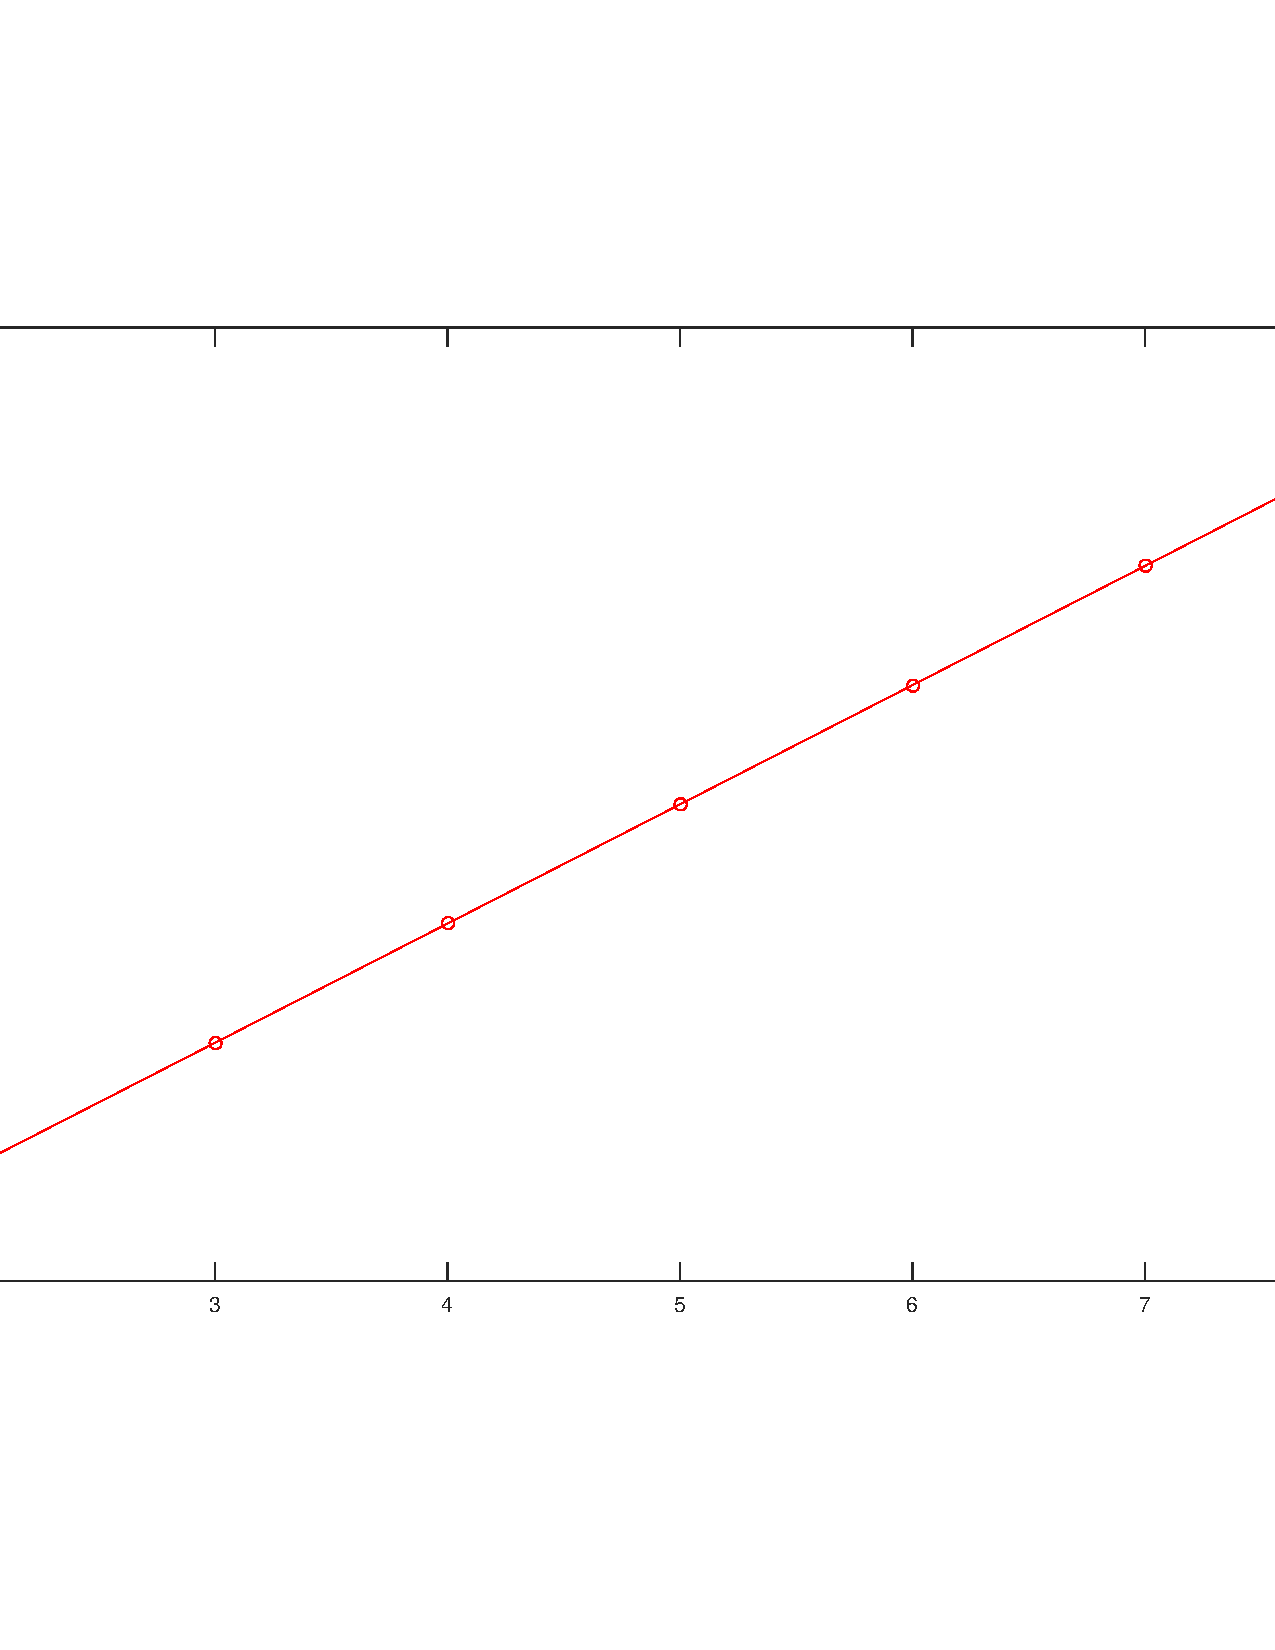
\includegraphics[width=\columnwidth]{replace_graph.pdf}}
 \caption{Plot of pneumatic cannon firing angle vs ending angle} 
 \label{fig:TradvsAutoDrop}
\end{figure}}
